\section{Auswertung und Analyse}
\begin{figure}[H]
    \centering
    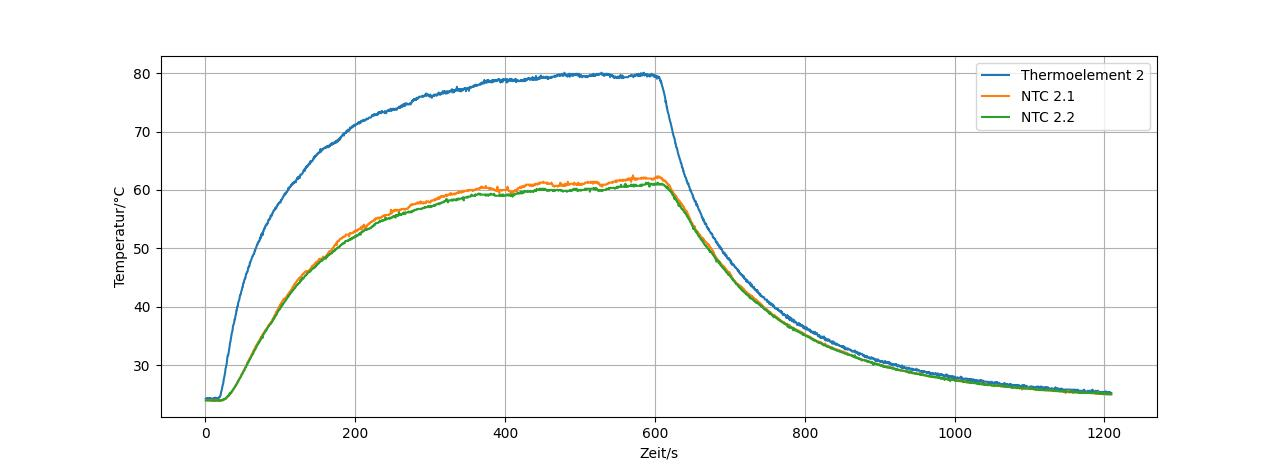
\includegraphics[width=0.9\textwidth]{data/temperatur_messung_mit_scheibe_16_00_.jpg}
    \caption{Temperaturverlauf mit Keramikscheibe}
    \label{fig:temperaturverlauf_mit_isolierung}
\end{figure}
\begin{figure}[H]
    \centering
    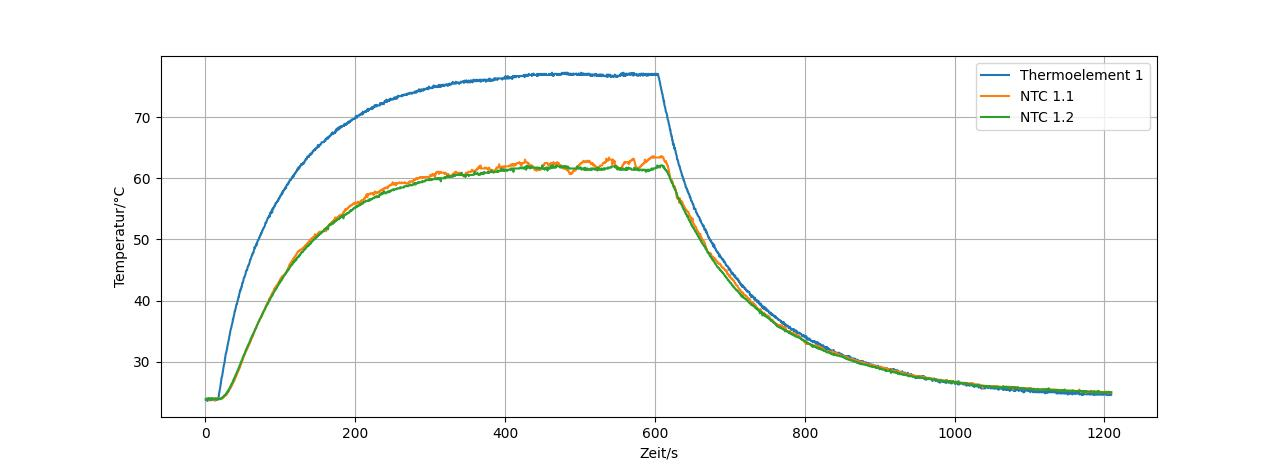
\includegraphics[width=0.9\textwidth]{data/temperatur_messung_ohne_scheibe_16_25_.jpg}
    \caption{Temperaturverlauf ohne Keramikscheibe}
    \label{fig:temperaturverlauf_ohne_isolierung}
\end{figure}

\subsection{Aufheizphase}
Die Aufheizphase erstreckt sich in einem Zeitberich von ca. \SI{15}{\second} bis \SI{610}{\second}. In diesem Zeitraum erwärmen sich die Transistoren von Raumtemperatur auf ihre Beharrungstemperatur.
Die Beharrungstemperatur geht aus aun Graphen der Messungen vor, dargestellt in Abbildung \ref{fig:temperaturverlauf_mit_isolierung} und Abbildung \ref{fig:temperaturverlauf_ohne_isolierung}.
\begin{table}[H]
    \centering
    \begin{tabular}{l|c|c}
        \toprule
        \textbf{Temperatursensor} & \textbf{Mit Isolierung}     & \textbf{Ohne Isolierung}    \\
        \midrule
        Thermoelement             & \SI{79.586}{\degreeCelsius} & \SI{76.913}{\degreeCelsius} \\
        NTC1                      & \SI{61.514}{\degreeCelsius} & \SI{62.528}{\degreeCelsius} \\
        NTC2                      & \SI{60.459}{\degreeCelsius} & \SI{61.539}{\degreeCelsius} \\
        \bottomrule
    \end{tabular}
    \caption{Beharrungstemperaturen der verschiedenen Sensoren}
    \label{tab:beharrungstemperaturen}
\end{table}
Wie in Kapitel \ref{sec:vorbereitung_aufgabe4} beschrieben, kann man nun beobachten wie lange es dauert, bis die Transistoren 63\% ihrer Beharrungstemperatur erreicht haben. Hierbei wird die Zeitkonstante $\tau$ bestimmt, indem die Kurve als PT2-System angenähert wird. Dafür wird das bereitgestellte Pythonprogramm zur Parameteridentifikation verwendet. Die Ergebnisse sind in Tabelle \ref{tab:taus} dargestellt.
\begin{table}[H]
    \centering
    \renewcommand{\arraystretch}{1.2}
    \begin{tabular}{lcccc}
        \toprule
                      & \multicolumn{2}{c}{\textbf{Mit Isolierung}} & \multicolumn{2}{c}{\textbf{Ohne Isolierung}}                                                      \\
        % \cmidrule(lr){2-3} draws a line only under columns 2 and 3 (trimmed Left and Right)
        \cmidrule(lr){2-3} \cmidrule(lr){4-5}
        Sensor        & $\tau$                                      & $T_{63\%}$                                   & $\tau$               & $T_{63\%}$                  \\
        \midrule
        Thermoelement & \SI{95.209}{\second}                        & \SI{59.105}{\degreeCelsius}                  & \SI{89.960}{\second} & \SI{57.263}{\degreeCelsius} \\
        NTC1          & \SI{112.264}{\second}                       & \SI{47.612}{\degreeCelsius}                  & \SI{95.062}{\second} & \SI{48.229}{\degreeCelsius} \\
        NTC2          & \SI{112.112}{\second}                       & \SI{46.951}{\degreeCelsius}                  & \SI{96.156}{\second} & \SI{47.610}{\degreeCelsius} \\
        \bottomrule
    \end{tabular}
    \caption{Zeitkonstanten und 63\%-Temperaturen der Aufheizphase}
    \label{tab:taus}
\end{table}
Hier kann man erkennen, dass die Zeitkonstanten bei dem Transistor mit Isolierung größer sind als bei dem Transistor ohne Isolierung. In einfachen Worten heißt es, dass der Transistor mit Isolierung sich langsamer aufheizt. Dies liegt daran, dass die Keramikscheibe die Wärmeabfuhr des Transistors erschwert, wodurch sich die Temperatur langsamer erhöht.
Das Programm nähert die Kurve als PT2-System an und gibt die Plotparameter aus, welche in Abbildung \ref{fig:plotparam_aufheiz_mit_isolierung_te} und Abbildung \ref{fig:plotparam_aufheiz_ohne_isolierung_te} dargestellt sind. Im prinzip werden die Parameter an der modellmäßg zu erwartenden Sprungantwort angepasst.
\begin{figure}[H]
    \centering
    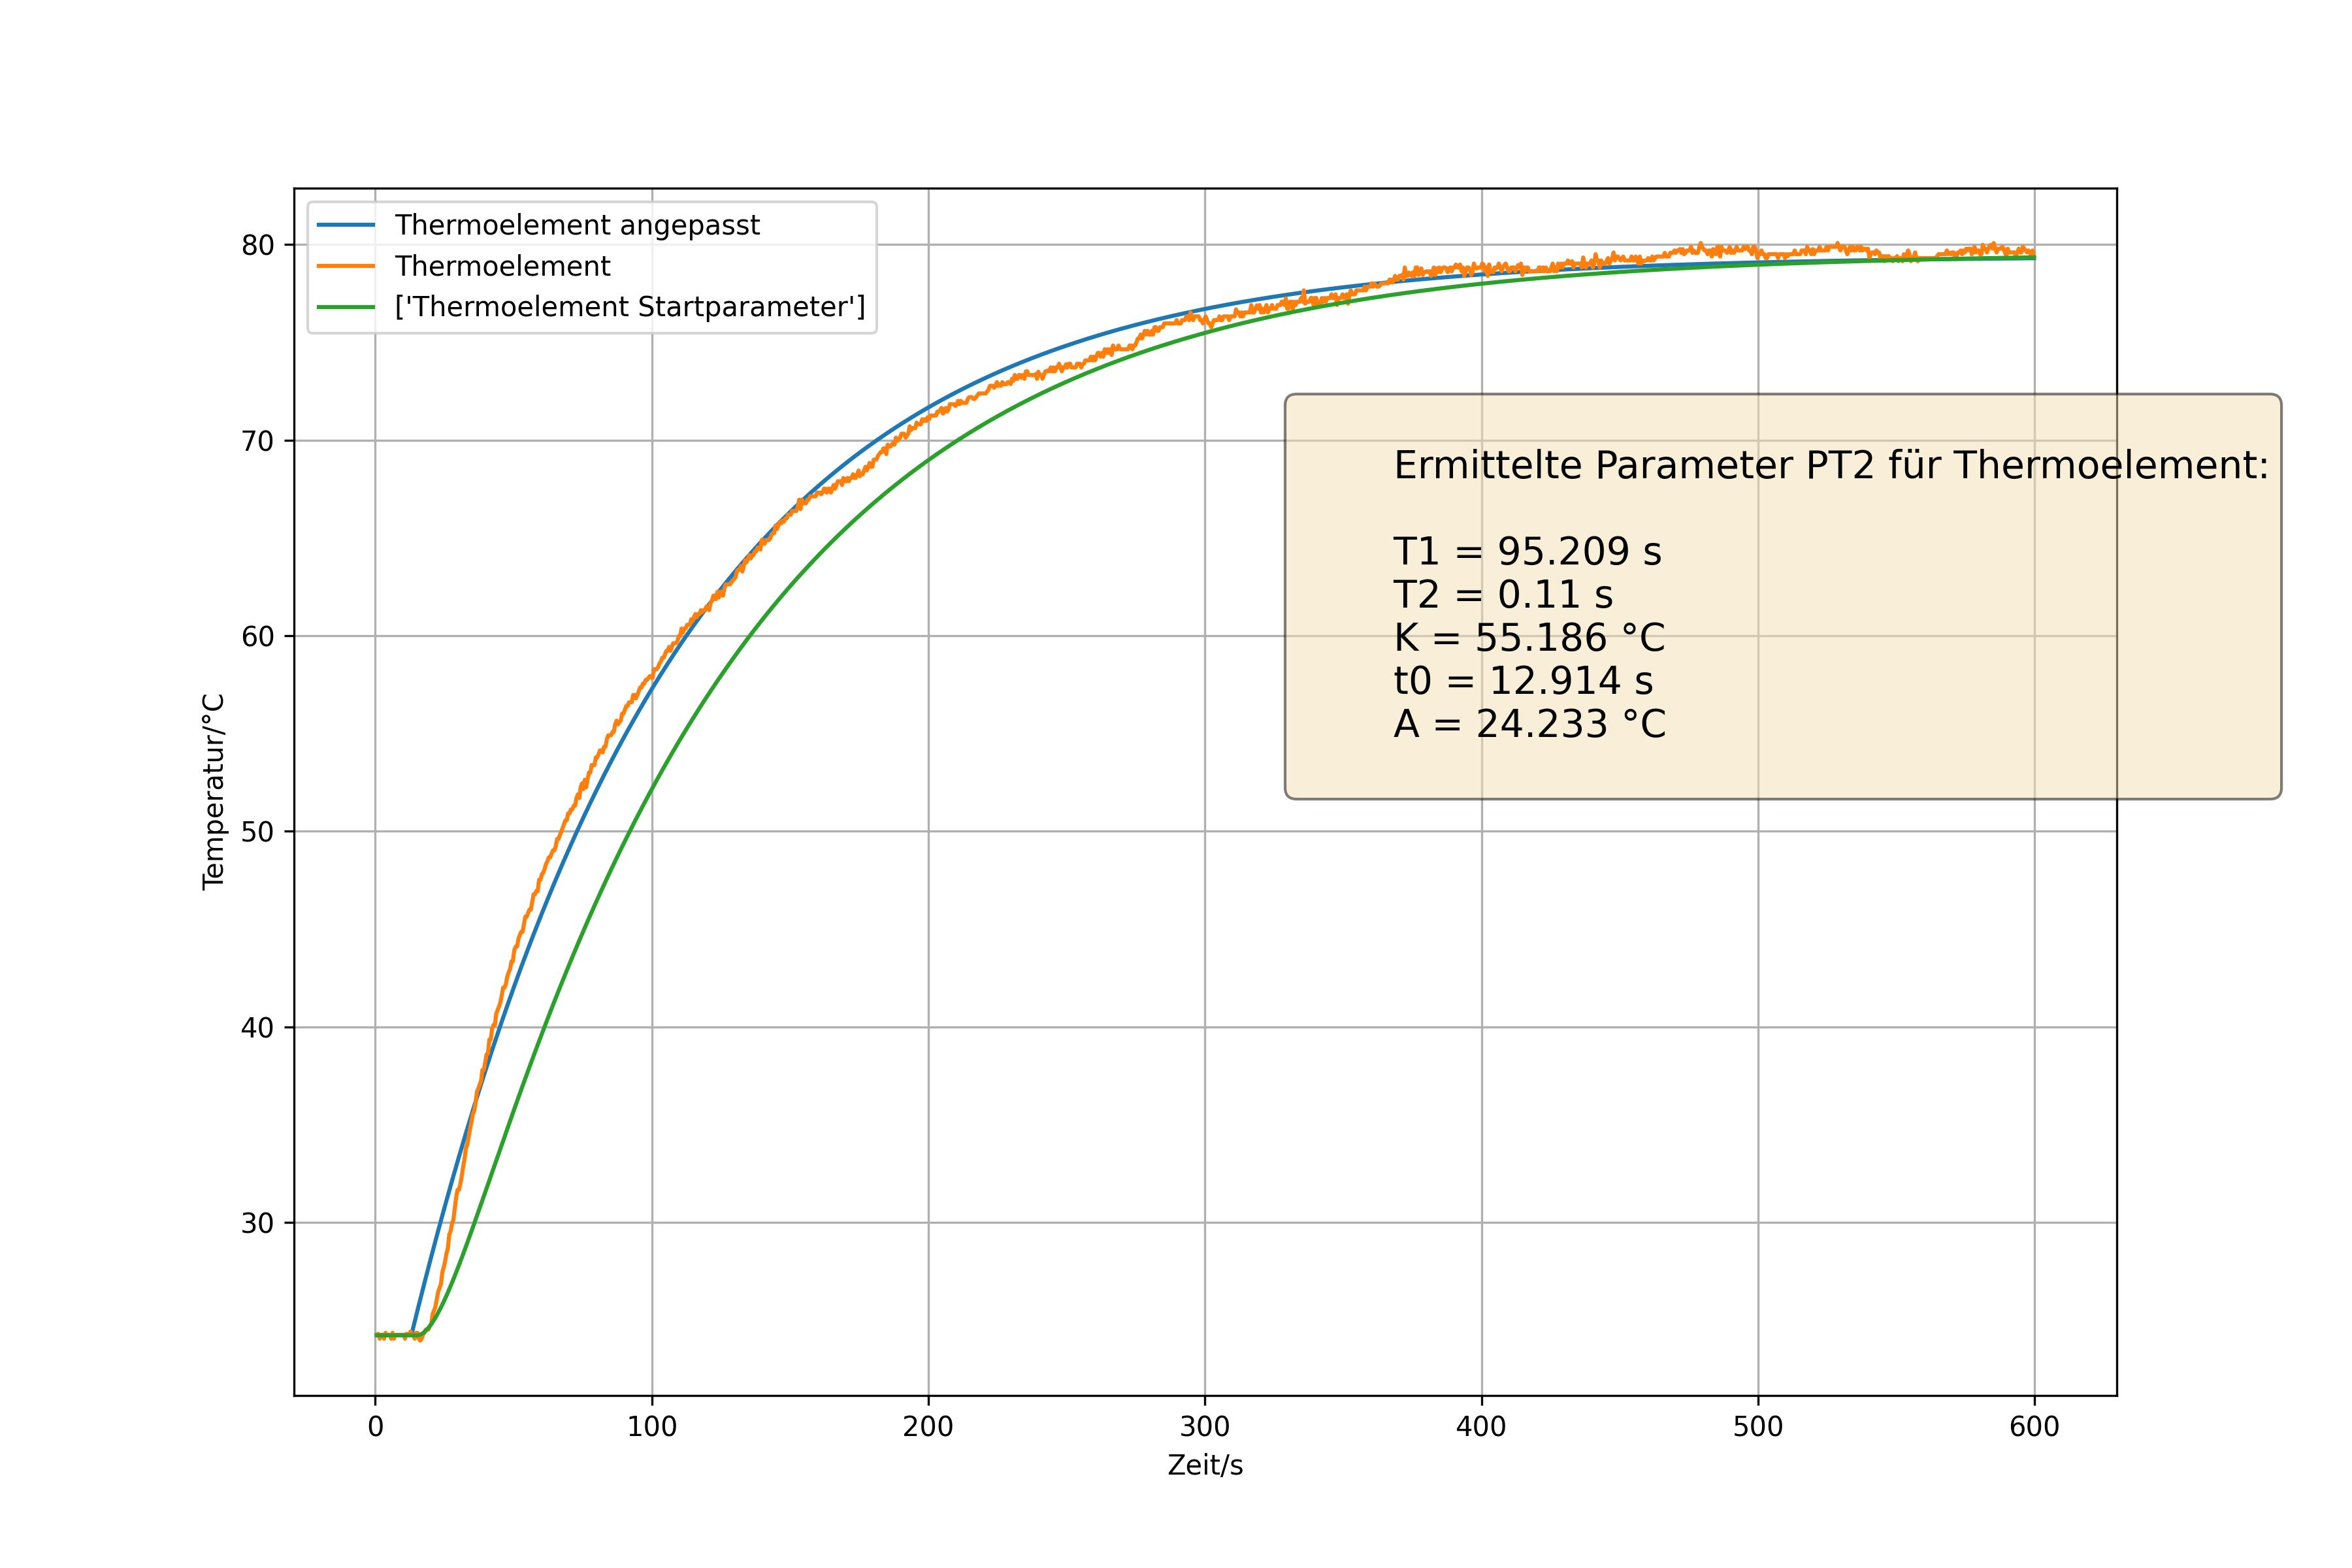
\includegraphics[width=0.9\textwidth]{data/auswertung/plotparameter_aufheiz_mit_scheibe16_19_00_TE_PT2.jpg}
    \caption{Plotparameter Aufheizphase mit Isolierung Thermoelement}
    \label{fig:plotparam_aufheiz_mit_isolierung_te}
\end{figure}
\begin{figure}[H]
    \centering
    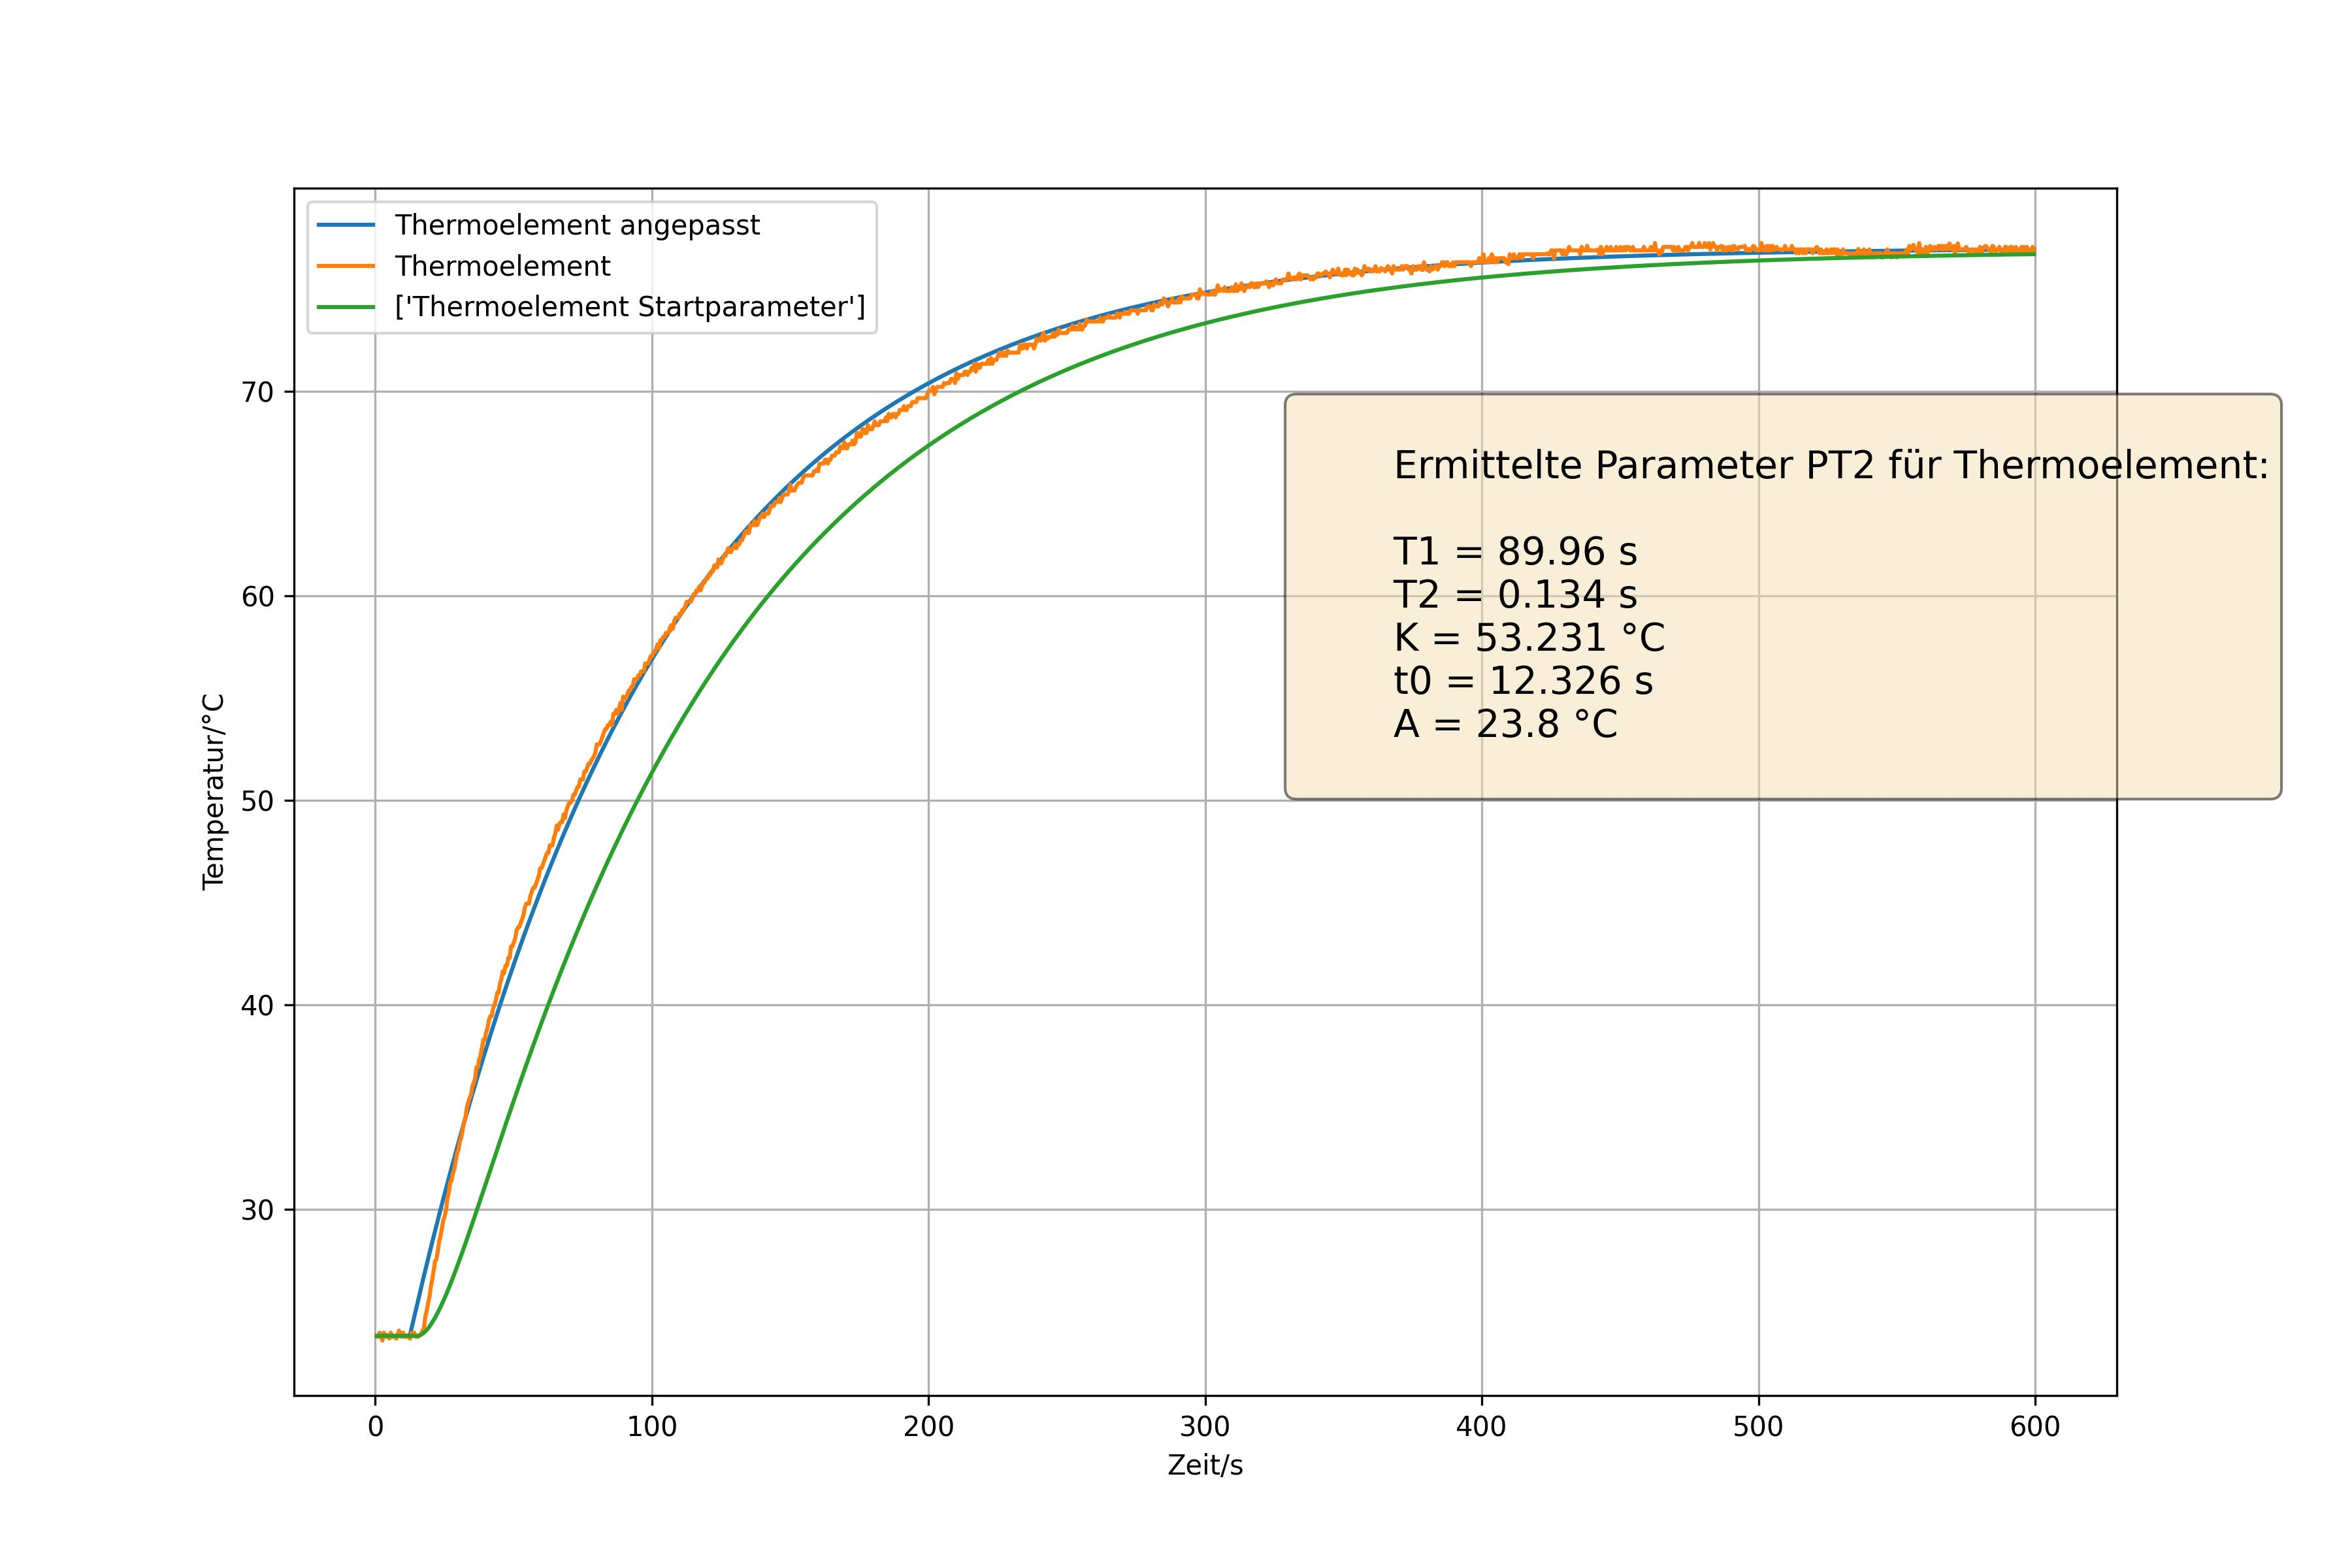
\includegraphics[width=0.9\textwidth]{data/auswertung/plotparameter_aufheiz_ohne_scheibe16_18_59_TE_PT2.jpg}
    \caption{Plotparameter Aufheizphase ohne Isolierung Thermoelement}
    \label{fig:plotparam_aufheiz_ohne_isolierung_te}
\end{figure}


\subsection{Abkühlphase}
Die Abkühlphase erstreckt sich in einem Zeitberich von ca. \SI{610}{\second} bis \SI{1220}{\second}. In diesem Zeitraum kühlen die Transistoren von ihrer Beharrungstemperatur wieder auf Raumtemperatur ab.
\begin{figure}[H]
    \centering
    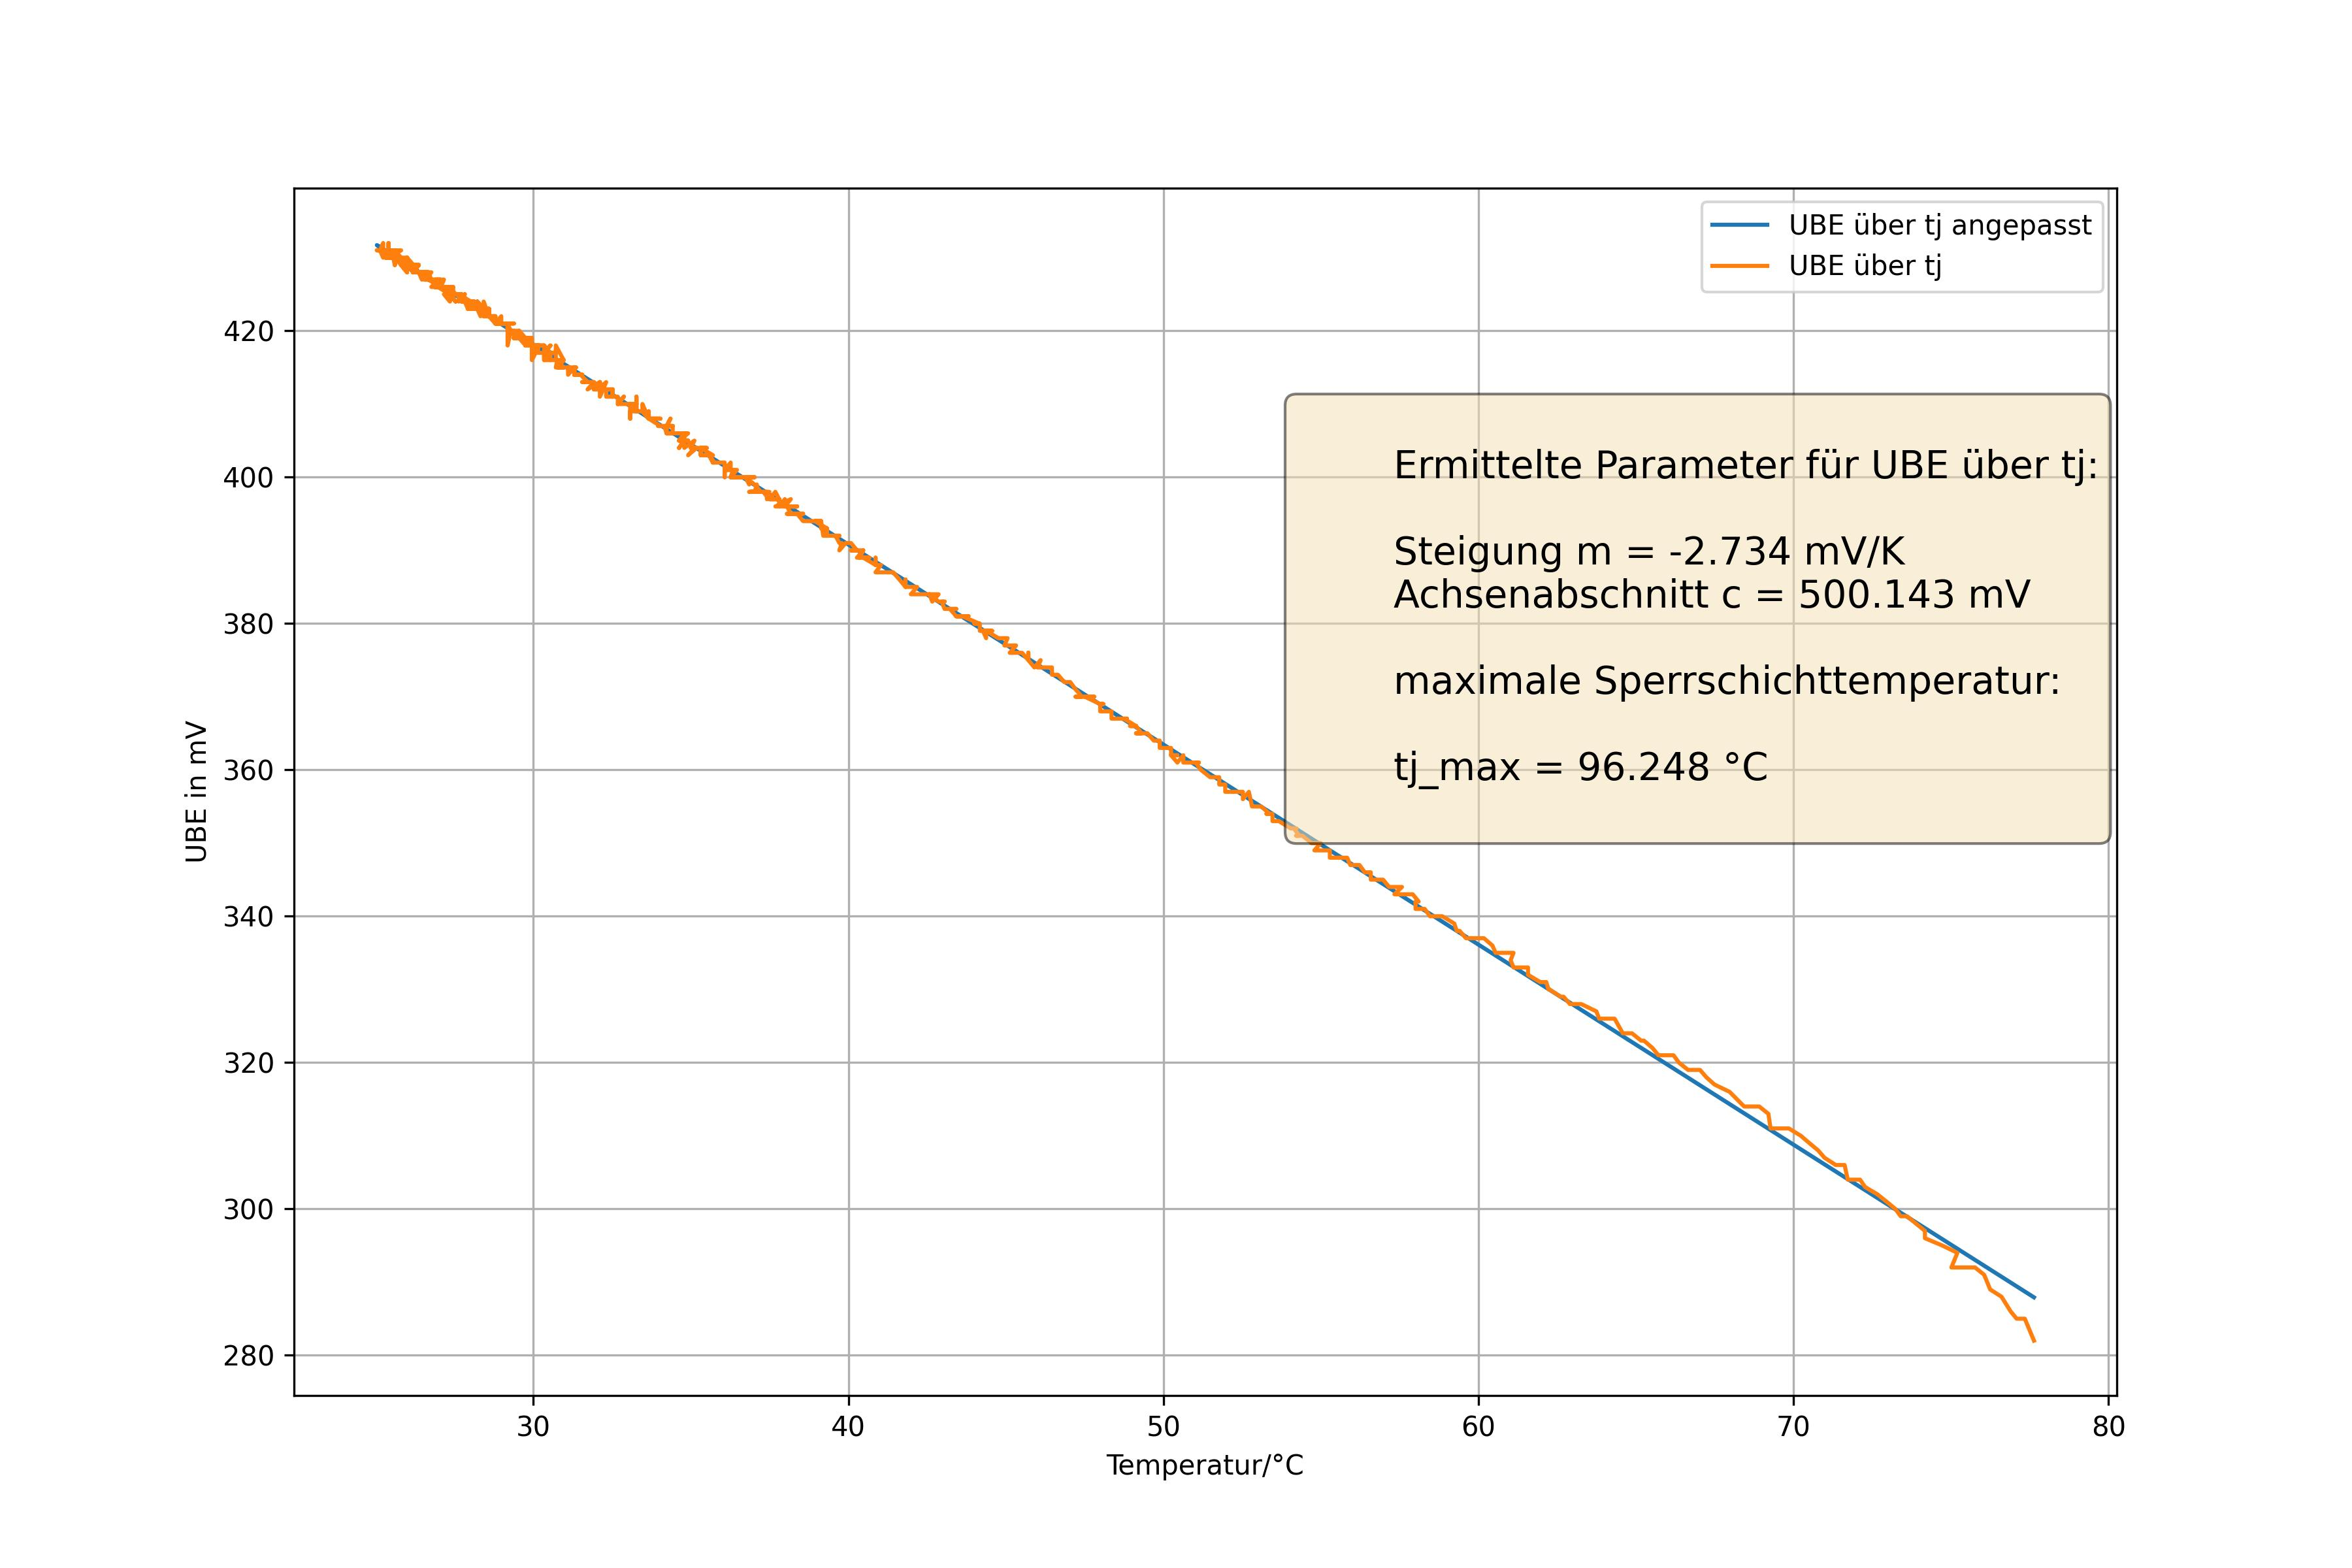
\includegraphics[width=0.9\textwidth]{data/auswertung/plotparameter_abkühl_mit_scheibe11_16_37_TE_Linear.jpg}
    \caption{Plotparameter Abkühlphase mit Isolierung Thermoelement}
    \label{fig:plotparam_abkuehl_mit_isolierung_te}
\end{figure}
\begin{figure}[H]
    \centering
    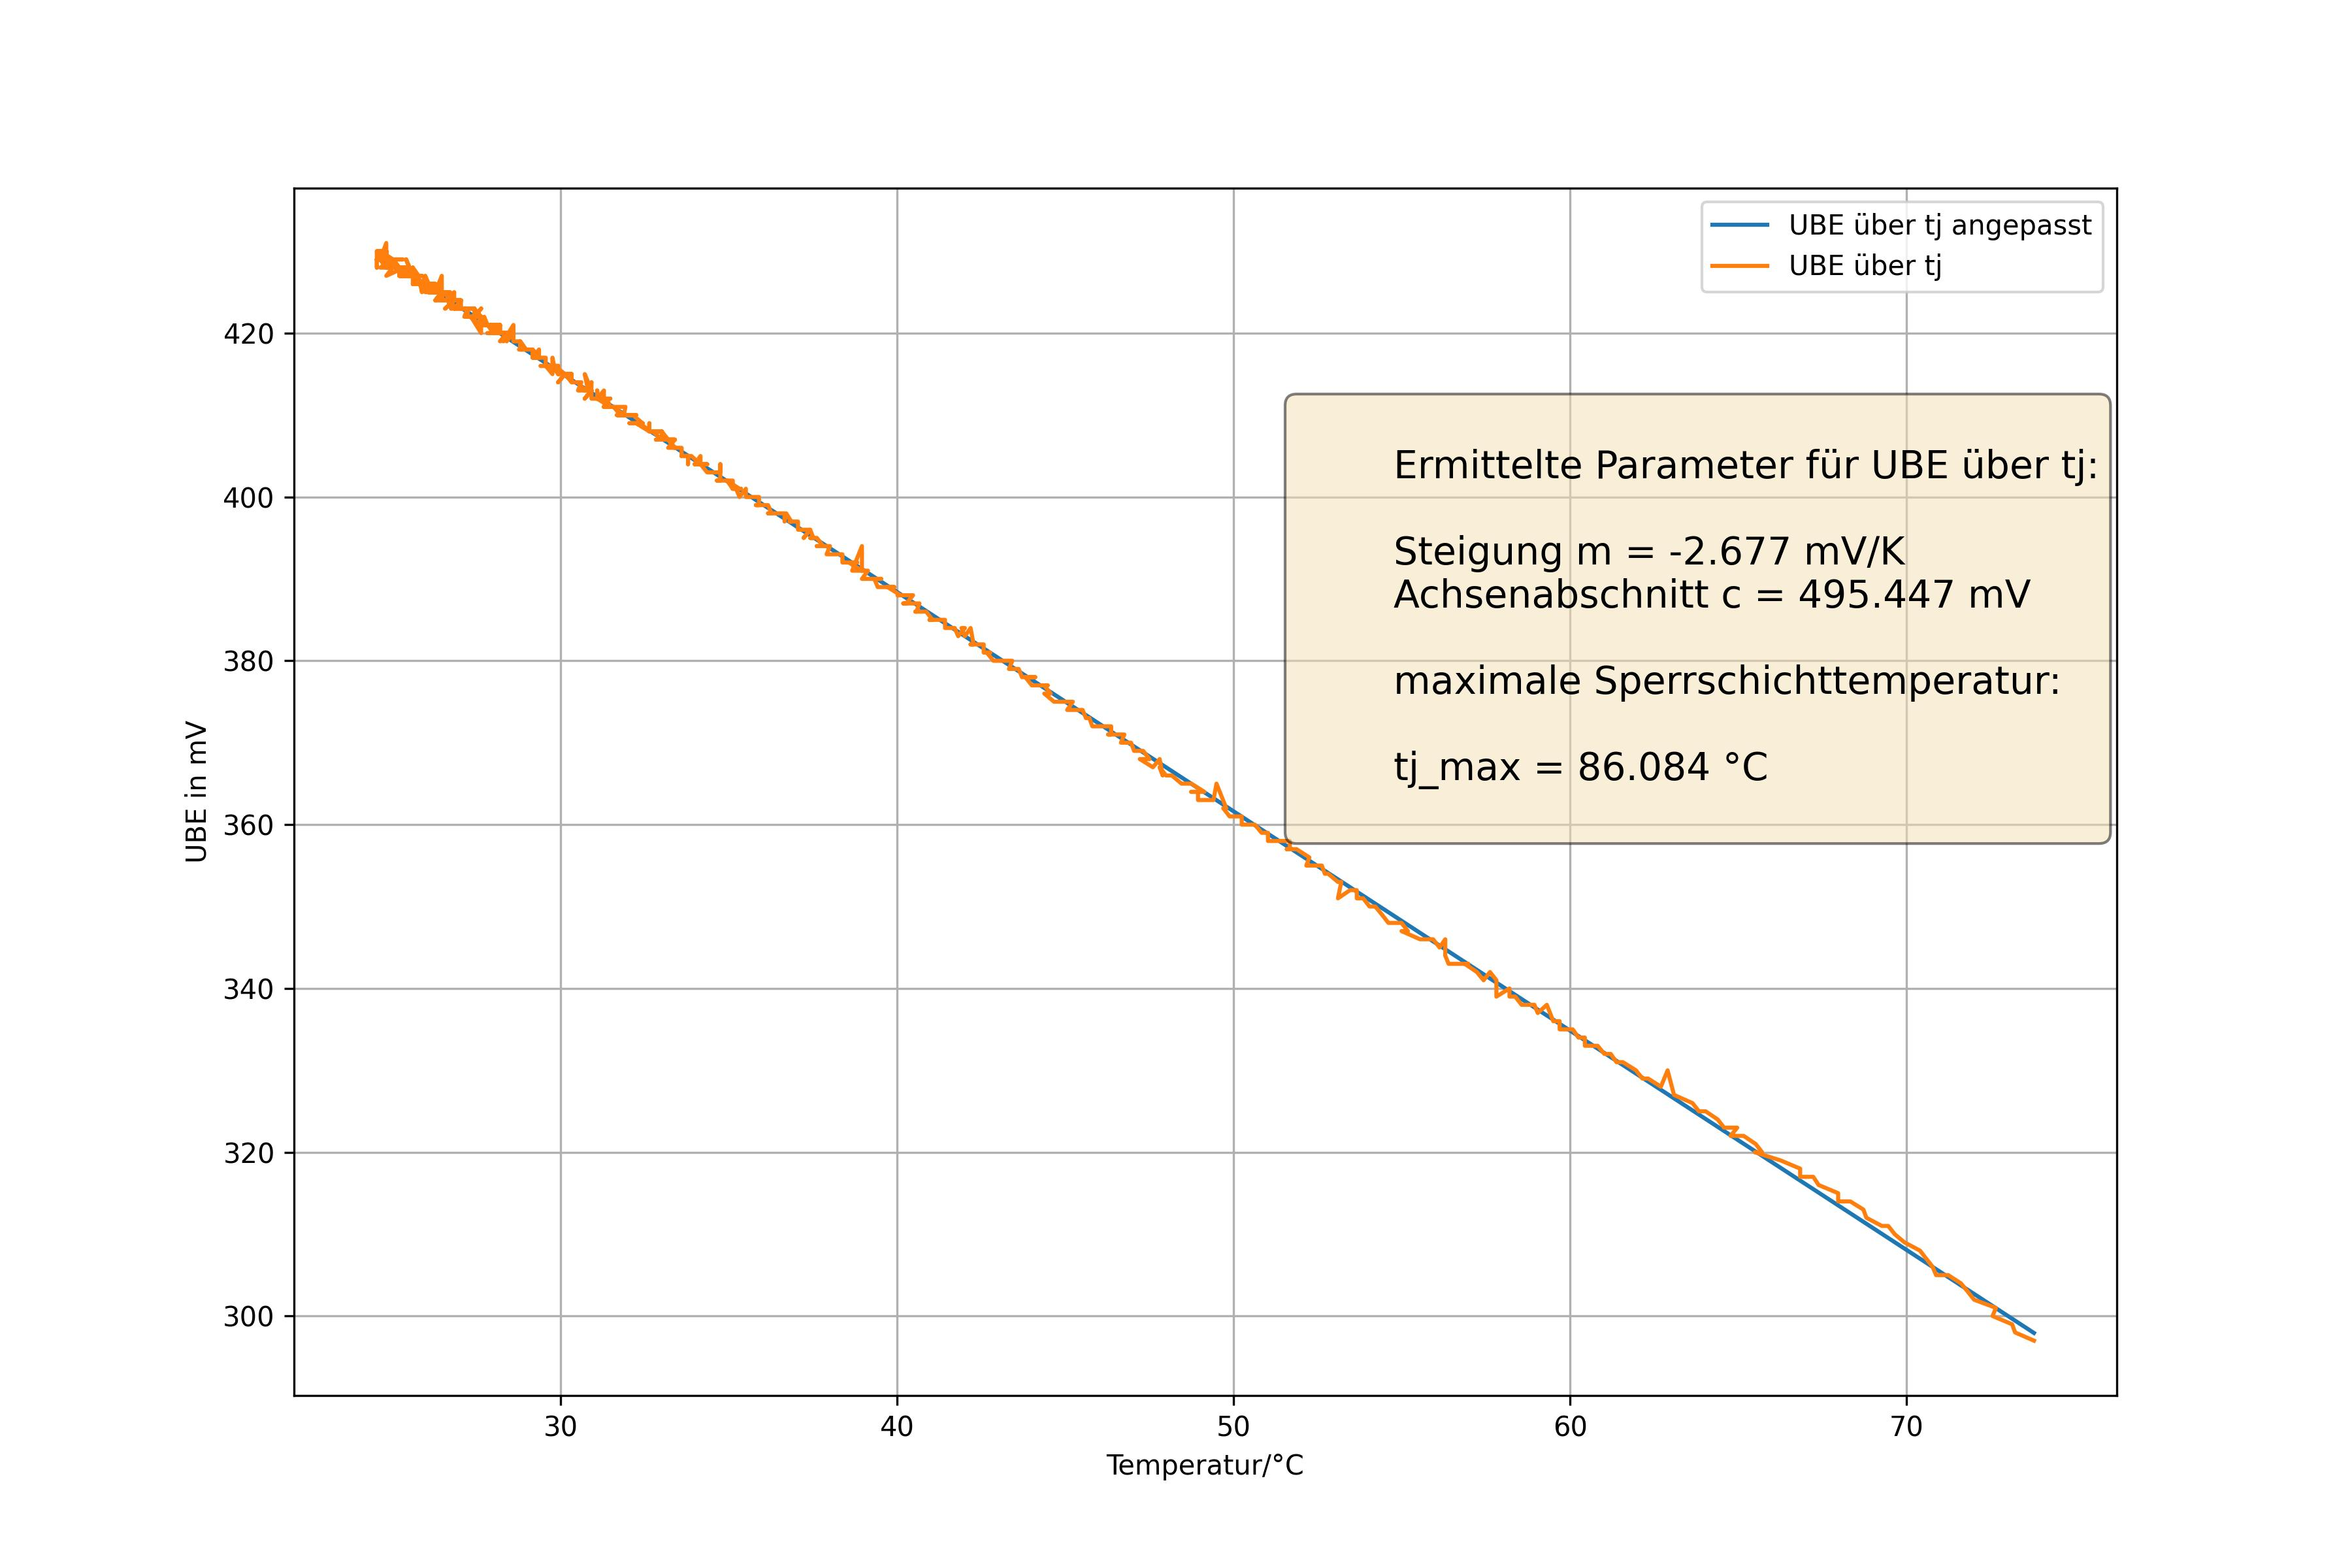
\includegraphics[width=0.9\textwidth]{data/auswertung/plotparameter_abkühl_ohne_scheibe11_16_36_TE_Linear.jpg}
    \caption{Plotparameter Abkühlphase ohne Isolierung Thermoelement}
    \label{fig:plotparam_abkuehl_ohne_isolierung_te}
\end{figure}

\subsection{Berechnung der Werte}

\subsubsection{Verlustleistung}
\label{scn:berechnung_verlustleistung}
Aus den Messdaten kann man die maximale $U_{CE}$ und $I_C$ Werte entnehmen:
\begin{equation}
    U_{CE} = \SI{2.93}{\volt}, \quad I_C = \SI{1.44}{\ampere}
\end{equation}
$U_{CE}$ und $I_C$ sind die maximalen Werte aus den Messdaten.
Damit ergibt sich die Verlustleistung zu:
\begin{equation}
    P_V = U_{CE} \cdot I_C = \SI{2.93}{\volt} \cdot \SI{1.44}{\ampere} = \boxed{\SI{4.2192}{\watt}}
\end{equation}

\subsubsection{Temperaturen}
\label{scn:anal_temp}
Die Kühlkörpertemperatur $\vartheta_S$ wird als Mittelwert der beiden NTC-Sensoren berechnet:
\begin{equation}
    \vartheta_S = \frac{\vartheta_{NTC1} + \vartheta_{NTC2}}{2}
\end{equation}
\begin{align*}
        \vartheta_S &= \frac{61.514 + 60.459}{2} \, \si{\degreeCelsius} = \boxed{\SI{60.9865}{\degreeCelsius}} \quad \text{(Mit Isolierung)} \\
        \vartheta_S &= \frac{62.528 + 61.539}{2} \, \si{\degreeCelsius} = \boxed{\SI{62.0335}{\degreeCelsius}} \quad \text{(Ohne Isolierung)}
\end{align*}
Die Gehäusetemperatur $\vartheta_C$ wird direkt aus dem Thermoelement abgelesen.
\begin{align*}
        \vartheta_C & = \boxed{\SI{79.586}{\degreeCelsius}} \quad \text{(Mit Isolierung)} \\
        \vartheta_C & = \boxed{\SI{76.913}{\degreeCelsius}} \quad \text{(Ohne Isolierung)}
\end{align*}
Um die maximale Sperrschichttemperatur $\vartheta_{J,max}$ zu bestimmen, wird die Temperaturabhängigkeit der Basis-Emitter-Spannung $U_{BE}$ genutzt. Da die Sperrschicht im Betrieb nicht direkt zugänglich ist, wird das Verhalten in der Abkühlphase analysiert. Nach dem Abschalten der Heizleistung gleichen sich die Sperrschichttemperatur $\vartheta_J$ und die Gehäusetemperatur $\vartheta_C$ schnell an, da kein Wärmestrom mehr von innen nach außen fließt. In diesem Zustand kann $\vartheta_C$ (gemessen mit dem Thermoelement) als Referenz für $\vartheta_J$ angenommen werden.

Mithilfe des Python-Programms wird eine lineare Regression durchgeführt, um die Kennlinie $U_{BE}(\vartheta) = m \cdot \vartheta + c$ zu bestimmen. Das Programm nutzt diese kalibrierte Kennlinie, um aus dem minimalen $U_{BE}$-Wert (gemessen unmittelbar beim Abschalten, als der Transistor am heißesten war) die maximale Sperrschichttemperatur $\vartheta_{J,max}$ zurückzurechnen.

Die ermittelten maximalen Sperrschichttemperaturen lauten:
\begin{align*}
    \vartheta_{J,max} &= \boxed{\SI{96.248}{\degreeCelsius}} \quad \text{(Mit Isolierung)} \\
    \vartheta_{J,max} &= \boxed{\SI{86.084}{\degreeCelsius}} \quad \text{(Ohne Isolierung)}
\end{align*}


\subsubsection{Wärmewirderstände}

Aus den ermittelten Beharrungstemperaturen und der elektrischen Verlustleistung $P_V$ lassen sich die Wärmewiderstände des Systems berechnen. Die Verlustleistung im stationären Zustand ergibt sich aus den Messdaten kurz vor dem Abschalten ($P_V = U_{CE} \cdot I_C$).

Die Wärmewiderstände berechnen sich analog zum Ohm'schen Gesetz aus der Temperaturdifferenz geteilt durch den Wärmestrom (Verlustleistung) :
\begin{align}
    R_{thJC} & = \frac{\vartheta_{J,max} - \vartheta_C}{P_V} \label{eq:RthJC} \\
    R_{thCS} & = \frac{\vartheta_C - \vartheta_S}{P_V} \label{eq:RthCS}       \\
    R_{thS}  & = \frac{\vartheta_S - \vartheta_U}{P_V} \label{eq:RthS}
\end{align}
Zur Ermittlung der Temperaturen siehe Abschnitt \ref{scn:anal_temp}.
\begin{align}
    R_{thJC} & = \frac{96.248 - 79.586}{4.2192} \, \si{\kelvin\per\watt} = \boxed{\SI{3.94}{\kelvin\per\watt}} \quad \text{(Mit Isolierung)} \\
    R_{thJC} & = \frac{86.084 - 76.913}{4.2192} \, \si{\kelvin\per\watt} = \boxed{\SI{2.18}{\kelvin\per\watt}} \quad \text{(Ohne Isolierung)} \\
    R_{thCS} & = \frac{79.586 - 60.9865}{4.2192} \, \si{\kelvin\per\watt} = \boxed{\SI{4.41}{\kelvin\per\watt}} \quad \text{(Mit Isolierung)} \\
    R_{thCS} & = \frac{76.913 - 62.0335}{4.2192} \, \si{\kelvin\per\watt} = \boxed{\SI{3.49}{\kelvin\per\watt}} \quad \text{(Ohne Isolierung)} \\
    R_{thS}  & = \frac{60.9865 - 22}{4.2192} \, \si{\kelvin\per\watt} = \boxed{\SI{9.26}{\kelvin\per\watt}} \quad \text{(Mit Isolierung)} \\
    R_{thS}  & = \frac{62.0335 - 22}{4.2192} \, \si{\kelvin\per\watt} = \boxed{\SI{9.52}{\kelvin\per\watt}} \quad \text{(Ohne Isolierung)}
\end{align}
\\
Tabelle \ref{tab:ergebnisse_gesamt} fasst die berechneten Parameter für beide Versuchsteile zusammen.

\subsection{Zusammenfassung der Ergebnisse}
\begin{table}[H]
    \centering
    \renewcommand{\arraystretch}{1.3}
    \begin{tabular}{l|c|c}
        \toprule
        \textbf{Parameter}                         & \textbf{Ohne Isolierscheibe}  & \textbf{Mit Isolierscheibe}   \\
        \midrule
        Verlustleistung $P_V$                      & \SI{4.2192}{\watt}            & \SI{4.2192}{\watt}            \\
        Kühlkörpertemp. $\vartheta_S$ (Mittelwert) & \SI{62.0335}{\degreeCelsius}  & \SI{60.9865}{\degreeCelsius}  \\
        Gehäusetemperatur $\vartheta_C$            & \SI{76.913}{\degreeCelsius}   & \SI{79.586}{\degreeCelsius}   \\
        Sperrschichttemperatur $\vartheta_{J,max}$ & \SI{86.084}{\degreeCelsius}   & \SI{96.248}{\degreeCelsius}   \\
        \midrule
        $R_{thJC}$ (Sperrschicht - Gehäuse)        & \SI{2.18}{\kelvin\per\watt}   & \SI{3.94}{\kelvin\per\watt}   \\
        $R_{thCS}$ (Gehäuse - Kühlkörper)          & \SI{3.49}{\kelvin\per\watt}   & \SI{4.41}{\kelvin\per\watt}   \\
        $R_{thS}$ (Kühlkörper - Umgebung)          & \SI{9.52}{\kelvin\per\watt}   & \SI{9.26}{\kelvin\per\watt}   \\
        \midrule
        Zeitkonstante $\tau$                       & \SI{89.960}{\second}          & \SI{95.209}{\second}          \\
        \bottomrule
    \end{tabular}
    \caption{Tabellarische Übersicht der messtechnisch ermittelten Parameter}
    \label{tab:ergebnisse_gesamt}
\end{table}
Die gemessenen Werte für die Wärmewiderstände weichen von den im Vorbereitungsteil berechneten Werten ab. Dies kann auf Messungenauigkeiten, Abweichungen in den Materialeigenschaften und vereinfachte Annahmen im theoretischen Modell zurückgeführt werden. Der Fehler wird in Kapitel \ref{scn:fehler_waermewiderstand} näher erläutert.